% Template for PLoS
% Version 3.4 January 2017
\documentclass[10pt,letterpaper]{article}
\usepackage[top=0.85in,left=2.75in,footskip=0.75in]{geometry}

% amsmath and amssymb packages, useful for mathematical formulas and symbols
\usepackage{amsmath,amssymb}

% Use adjustwidth environment to exceed column width (see example table in text)
\usepackage{changepage}

% Use Unicode characters when possible
\usepackage[utf8x]{inputenc}

% textcomp package and marvosym package for additional characters
\usepackage{textcomp,marvosym}

% cite package, to clean up citations in the main text. Do not remove.
% \usepackage{cite}

% Use nameref to cite supporting information files (see Supporting Information section for more info)
\usepackage{nameref,hyperref}

% line numbers
\usepackage[right]{lineno}

% ligatures disabled
\usepackage{microtype}
\DisableLigatures[f]{encoding = *, family = * }

% color can be used to apply background shading to table cells only
\usepackage[table]{xcolor}

% array package and thick rules for tables
\usepackage{array}

% create "+" rule type for thick vertical lines
\newcolumntype{+}{!{\vrule width 2pt}}

% create \thickcline for thick horizontal lines of variable length
\newlength\savedwidth
\newcommand\thickcline[1]{%
  \noalign{\global\savedwidth\arrayrulewidth\global\arrayrulewidth 2pt}%
  \cline{#1}%
  \noalign{\vskip\arrayrulewidth}%
  \noalign{\global\arrayrulewidth\savedwidth}%
}

% \thickhline command for thick horizontal lines that span the table
\newcommand\thickhline{\noalign{\global\savedwidth\arrayrulewidth\global\arrayrulewidth 2pt}%
\hline
\noalign{\global\arrayrulewidth\savedwidth}}


% Remove comment for double spacing
%\usepackage{setspace} 
%\doublespacing

% Text layout
\raggedright
\setlength{\parindent}{0.5cm}
\textwidth 5.25in 
\textheight 8.75in

% Bold the 'Figure #' in the caption and separate it from the title/caption with a period
% Captions will be left justified
\usepackage[aboveskip=1pt,labelfont=bf,labelsep=period,justification=raggedright,singlelinecheck=off]{caption}
\renewcommand{\figurename}{Fig}

% Use the PLoS provided BiBTeX style
% \bibliographystyle{plos2015}

% Remove brackets from numbering in List of References
\makeatletter
\renewcommand{\@biblabel}[1]{\quad#1.}
\makeatother

% Leave date blank
\date{}

% Header and Footer with logo
\usepackage{lastpage,fancyhdr,graphicx}
\usepackage{epstopdf}
\pagestyle{myheadings}
\pagestyle{fancy}
\fancyhf{}
\setlength{\headheight}{27.023pt}
\lhead{
\includegraphics[width=2.0in]{PLOS-submission.eps}}
\rfoot{\thepage/\pageref{LastPage}}
\renewcommand{\footrule}{\hrule height 2pt \vspace{2mm}}
\fancyheadoffset[L]{2.25in}
\fancyfootoffset[L]{2.25in}
\lfoot{\sf PLOS}

%% Include all macros below
\newcommand{\lorem}{{\bf LOREM}}
\newcommand{\ipsum}{{\bf IPSUM}}

\usepackage{color}
\usepackage{fancyvrb}
\newcommand{\VerbBar}{|}
\newcommand{\VERB}{\Verb[commandchars=\\\{\}]}
\DefineVerbatimEnvironment{Highlighting}{Verbatim}{commandchars=\\\{\}}
% Add ',fontsize=\small' for more characters per line
\usepackage{framed}
\definecolor{shadecolor}{RGB}{248,248,248}
\newenvironment{Shaded}{\begin{snugshade}}{\end{snugshade}}
\newcommand{\KeywordTok}[1]{\textcolor[rgb]{0.13,0.29,0.53}{\textbf{#1}}}
\newcommand{\DataTypeTok}[1]{\textcolor[rgb]{0.13,0.29,0.53}{#1}}
\newcommand{\DecValTok}[1]{\textcolor[rgb]{0.00,0.00,0.81}{#1}}
\newcommand{\BaseNTok}[1]{\textcolor[rgb]{0.00,0.00,0.81}{#1}}
\newcommand{\FloatTok}[1]{\textcolor[rgb]{0.00,0.00,0.81}{#1}}
\newcommand{\ConstantTok}[1]{\textcolor[rgb]{0.00,0.00,0.00}{#1}}
\newcommand{\CharTok}[1]{\textcolor[rgb]{0.31,0.60,0.02}{#1}}
\newcommand{\SpecialCharTok}[1]{\textcolor[rgb]{0.00,0.00,0.00}{#1}}
\newcommand{\StringTok}[1]{\textcolor[rgb]{0.31,0.60,0.02}{#1}}
\newcommand{\VerbatimStringTok}[1]{\textcolor[rgb]{0.31,0.60,0.02}{#1}}
\newcommand{\SpecialStringTok}[1]{\textcolor[rgb]{0.31,0.60,0.02}{#1}}
\newcommand{\ImportTok}[1]{#1}
\newcommand{\CommentTok}[1]{\textcolor[rgb]{0.56,0.35,0.01}{\textit{#1}}}
\newcommand{\DocumentationTok}[1]{\textcolor[rgb]{0.56,0.35,0.01}{\textbf{\textit{#1}}}}
\newcommand{\AnnotationTok}[1]{\textcolor[rgb]{0.56,0.35,0.01}{\textbf{\textit{#1}}}}
\newcommand{\CommentVarTok}[1]{\textcolor[rgb]{0.56,0.35,0.01}{\textbf{\textit{#1}}}}
\newcommand{\OtherTok}[1]{\textcolor[rgb]{0.56,0.35,0.01}{#1}}
\newcommand{\FunctionTok}[1]{\textcolor[rgb]{0.00,0.00,0.00}{#1}}
\newcommand{\VariableTok}[1]{\textcolor[rgb]{0.00,0.00,0.00}{#1}}
\newcommand{\ControlFlowTok}[1]{\textcolor[rgb]{0.13,0.29,0.53}{\textbf{#1}}}
\newcommand{\OperatorTok}[1]{\textcolor[rgb]{0.81,0.36,0.00}{\textbf{#1}}}
\newcommand{\BuiltInTok}[1]{#1}
\newcommand{\ExtensionTok}[1]{#1}
\newcommand{\PreprocessorTok}[1]{\textcolor[rgb]{0.56,0.35,0.01}{\textit{#1}}}
\newcommand{\AttributeTok}[1]{\textcolor[rgb]{0.77,0.63,0.00}{#1}}
\newcommand{\RegionMarkerTok}[1]{#1}
\newcommand{\InformationTok}[1]{\textcolor[rgb]{0.56,0.35,0.01}{\textbf{\textit{#1}}}}
\newcommand{\WarningTok}[1]{\textcolor[rgb]{0.56,0.35,0.01}{\textbf{\textit{#1}}}}
\newcommand{\AlertTok}[1]{\textcolor[rgb]{0.94,0.16,0.16}{#1}}
\newcommand{\ErrorTok}[1]{\textcolor[rgb]{0.64,0.00,0.00}{\textbf{#1}}}
\newcommand{\NormalTok}[1]{#1}




\usepackage{forarray}
\usepackage{xstring}
\newcommand{\getIndex}[2]{
  \ForEach{,}{\IfEq{#1}{\thislevelitem}{\number\thislevelcount\ExitForEach}{}}{#2}
}

\setcounter{secnumdepth}{0}

\newcommand{\getAff}[1]{
  \getIndex{#1}{Michigan State University,Michigan State University}
}

\providecommand{\tightlist}{%
  \setlength{\itemsep}{0pt}\setlength{\parskip}{0pt}}

\begin{document}
\vspace*{0.2in}

% Title must be 250 characters or less.
\begin{flushleft}
{\Large
\textbf\newline{Title of submission to PLOS journal} % Please use "sentence case" for title and headings (capitalize only the first word in a title (or heading), the first word in a subtitle (or subheading), and any proper nouns).
}
\newline
\\
Sean L. Nguyen\textsuperscript{\getAff{Michigan State University}},
Margaret G. Petroff\textsuperscript{\getAff{Michigan State University}}\textsuperscript{*}\\
\bigskip
\textbf{\getAff{Michigan State University}}Program in Cell and Molecular Biology, 474 S Shaw Ln, East lansing, MI,
48824\\
\textbf{\getAff{Michigan State University}}Department of Pathobiology and Diagnostic Investigation, 784 Wilson Rd,
East Lansing, MI, 48824\\
\bigskip
* Corresponding author: petrof10@msu.edu\\
\end{flushleft}
% Please keep the abstract below 300 words
\section*{Abstract}
Lorem ipsum dolor sit amet, consectetur adipiscing elit. Curabitur eget
porta erat. Morbi consectetur est vel gravida pretium. Suspendisse ut
dui eu ante cursus gravida non sed sem. Nullam sapien tellus, commodo id
velit id, eleifend volutpat quam. Phasellus mauris velit, dapibus
finibus elementum vel, pulvinar non tellus. Nunc pellentesque pretium
diam, quis maximus dolor faucibus id. Nunc convallis sodales ante, ut
ullamcorper est egestas vitae. Nam sit amet enim ultrices, ultrices elit
pulvinar, volutpat risus.

% Please keep the Author Summary between 150 and 200 words
% Use first person. PLOS ONE authors please skip this step. 
% Author Summary not valid for PLOS ONE submissions.   
\section*{Author summary}
Lorem ipsum dolor sit amet, consectetur adipiscing elit. Curabitur eget
porta erat. Morbi consectetur est vel gravida pretium. Suspendisse ut
dui eu ante cursus gravida non sed sem. Nullam sapien tellus, commodo id
velit id, eleifend volutpat quam. Phasellus mauris velit, dapibus
finibus elementum vel, pulvinar non tellus. Nunc pellentesque pretium
diam, quis maximus dolor faucibus id. Nunc convallis sodales ante, ut
ullamcorper est egestas vitae. Nam sit amet enim ultrices, ultrices elit
pulvinar, volutpat risus.

\linenumbers

% Use "Eq" instead of "Equation" for equation citations.
\emph{Text based on plos sample manuscript, see
\url{http://journals.plos.org/ploscompbiol/s/latex}}

\section{Introduction}\label{introduction}

Lorem ipsum dolor sit amet, consectetur adipiscing elit. Curabitur eget
porta erat. Morbi consectetur est vel gravida pretium. Suspendisse ut
dui eu ante cursus gravida non sed sem. Phasellus mauris velit, dapibus
finibus elementum vel, pulvinar non tellus. Nunc pellentesque pretium
diam, quis maximus dolor faucibus id. Nunc convallis sodales ante, ut
ullamcorper est egestas vitae. Nam sit amet enim ultrices, ultrices elit
pulvinar, volutpat risus.

A list

\begin{itemize}
\tightlist
\item
  Item 1
\item
  Item 2
\end{itemize}

\begin{Shaded}
\begin{Highlighting}[]
\KeywordTok{library}\NormalTok{(tidyverse)}

\NormalTok{file <-}\StringTok{ "nanosight_data.csv"}


\NormalTok{raw_data <-}\StringTok{ }\KeywordTok{read_csv}\NormalTok{(file)}
\NormalTok{raw_data}
\end{Highlighting}
\end{Shaded}

\begin{verbatim}
## # A tibble: 1,000 x 37
##    particle_size mG15.5_yes_500_00 mG15.5_yes_500_01 mG15.5_yes_500_02
##            <dbl>             <int>             <int>             <int>
##  1         0.500                 0                 0                 0
##  2         1.50                  0                 0                 0
##  3         2.50                  0                 0                 0
##  4         3.50                  0                 0                 0
##  5         4.50                  0                 0                 0
##  6         5.50                  0                 0                 0
##  7         6.50                  0                 0                 0
##  8         7.50                  0                 0                 0
##  9         8.50                  0                 0                 0
## 10         9.50                  0                 0                 0
## # ... with 990 more rows, and 33 more variables: mG15.5_no_500_00 <int>,
## #   mG15.5_no_500_01 <int>, mG15.5_no_500_02 <int>, `400_yes_50_00` <int>,
## #   `400_yes_50_01` <int>, `400_yes_50_02` <int>, `400_no_50_00` <int>,
## #   `400_no_50_01` <int>, `400_no_50_02` <int>, `200_yes_125_00` <int>,
## #   `200_yes_125_01` <int>, `200_yes_125_02` <int>, `200_no_125_00` <int>,
## #   `200_no_125_01` <int>, `200_no_125_02` <int>,
## #   fluorx100_no_125_00 <int>, fluorx100_no_125_01 <int>,
## #   fluorx100_no_125_02 <int>, fluorx100_yes_125_00 <int>,
## #   fluorx100_yes_125_01 <int>, fluorx100_yes_125_02 <int>,
## #   fluor_no_125_00 <int>, fluor_no_125_01 <int>, fluor_no_125_02 <int>,
## #   fluor_yes_125_00 <int>, fluor_yes_125_01 <int>,
## #   fluor_yes_125_02 <int>, `100_no_125_00` <int>, `100_no_125_01` <int>,
## #   `100_no_125_02` <int>, `100_yes_125_00` <int>, `100_yes_125_01` <int>,
## #   `100_yes_125_02` <int>
\end{verbatim}

\begin{Shaded}
\begin{Highlighting}[]
\NormalTok{raw_data }\OperatorTok\StringTok{ }
\StringTok{  }\KeywordTok{gather}\NormalTok{(ID,values,}\DecValTok{2}\OperatorTok{:}\DecValTok{37}\NormalTok{)}
\end{Highlighting}
\end{Shaded}

\begin{verbatim}
## # A tibble: 36,000 x 3
##    particle_size ID                values
##            <dbl> <chr>              <int>
##  1         0.500 mG15.5_yes_500_00      0
##  2         1.50  mG15.5_yes_500_00      0
##  3         2.50  mG15.5_yes_500_00      0
##  4         3.50  mG15.5_yes_500_00      0
##  5         4.50  mG15.5_yes_500_00      0
##  6         5.50  mG15.5_yes_500_00      0
##  7         6.50  mG15.5_yes_500_00      0
##  8         7.50  mG15.5_yes_500_00      0
##  9         8.50  mG15.5_yes_500_00      0
## 10         9.50  mG15.5_yes_500_00      0
## # ... with 35,990 more rows
\end{verbatim}

\begin{Shaded}
\begin{Highlighting}[]
\NormalTok{raw_data }\OperatorTok\StringTok{ }
\StringTok{  }\KeywordTok{gather}\NormalTok{(ID,values,}\DecValTok{2}\OperatorTok{:}\DecValTok{37}\NormalTok{) }\OperatorTok\StringTok{ }
\StringTok{  }\KeywordTok{separate}\NormalTok{(ID, }\DataTypeTok{into =} \KeywordTok{c}\NormalTok{(}\StringTok{"sample"}\NormalTok{, }\StringTok{"filter"}\NormalTok{, }\StringTok{"dilution_factor"}\NormalTok{,}\StringTok{"tech_rep"}\NormalTok{), }\DataTypeTok{sep =} \StringTok{"_"}\NormalTok{)}
\end{Highlighting}
\end{Shaded}

\begin{verbatim}
## # A tibble: 36,000 x 6
##    particle_size sample filter dilution_factor tech_rep values
##            <dbl> <chr>  <chr>  <chr>           <chr>     <int>
##  1         0.500 mG15.5 yes    500             00            0
##  2         1.50  mG15.5 yes    500             00            0
##  3         2.50  mG15.5 yes    500             00            0
##  4         3.50  mG15.5 yes    500             00            0
##  5         4.50  mG15.5 yes    500             00            0
##  6         5.50  mG15.5 yes    500             00            0
##  7         6.50  mG15.5 yes    500             00            0
##  8         7.50  mG15.5 yes    500             00            0
##  9         8.50  mG15.5 yes    500             00            0
## 10         9.50  mG15.5 yes    500             00            0
## # ... with 35,990 more rows
\end{verbatim}

\begin{Shaded}
\begin{Highlighting}[]
\NormalTok{raw_data }\OperatorTok\StringTok{ }
\StringTok{  }\KeywordTok{gather}\NormalTok{(ID,values,}\DecValTok{2}\OperatorTok{:}\DecValTok{37}\NormalTok{) }\OperatorTok\StringTok{ }
\StringTok{  }\KeywordTok{separate}\NormalTok{(ID, }\DataTypeTok{into =} \KeywordTok{c}\NormalTok{(}\StringTok{"sample"}\NormalTok{, }\StringTok{"filter"}\NormalTok{, }\StringTok{"dilution_factor"}\NormalTok{,}\StringTok{"tech_rep"}\NormalTok{), }\DataTypeTok{sep =} \StringTok{"_"}\NormalTok{) }\OperatorTok\StringTok{ }
\StringTok{  }\KeywordTok{mutate_at}\NormalTok{(}\KeywordTok{vars}\NormalTok{(sample,filter,tech_rep),as.factor) }\OperatorTok\StringTok{ }
\StringTok{  }\KeywordTok{mutate_at}\NormalTok{(}\KeywordTok{vars}\NormalTok{(dilution_factor),as.numeric)}
\end{Highlighting}
\end{Shaded}

\begin{verbatim}
## # A tibble: 36,000 x 6
##    particle_size sample filter dilution_factor tech_rep values
##            <dbl> <fct>  <fct>            <dbl> <fct>     <int>
##  1         0.500 mG15.5 yes                500 00            0
##  2         1.50  mG15.5 yes                500 00            0
##  3         2.50  mG15.5 yes                500 00            0
##  4         3.50  mG15.5 yes                500 00            0
##  5         4.50  mG15.5 yes                500 00            0
##  6         5.50  mG15.5 yes                500 00            0
##  7         6.50  mG15.5 yes                500 00            0
##  8         7.50  mG15.5 yes                500 00            0
##  9         8.50  mG15.5 yes                500 00            0
## 10         9.50  mG15.5 yes                500 00            0
## # ... with 35,990 more rows
\end{verbatim}

\begin{Shaded}
\begin{Highlighting}[]
\NormalTok{data <-}\StringTok{ }\NormalTok{raw_data }\OperatorTok\StringTok{ }
\StringTok{  }\KeywordTok{gather}\NormalTok{(ID,values,}\DecValTok{2}\OperatorTok{:}\DecValTok{37}\NormalTok{) }\OperatorTok\StringTok{ }
\StringTok{  }\KeywordTok{separate}\NormalTok{(ID, }\DataTypeTok{into =} \KeywordTok{c}\NormalTok{(}\StringTok{"sample"}\NormalTok{, }\StringTok{"filter"}\NormalTok{, }\StringTok{"dilution_factor"}\NormalTok{,}\StringTok{"tech_rep"}\NormalTok{), }\DataTypeTok{sep =} \StringTok{"_"}\NormalTok{) }\OperatorTok\StringTok{ }
\StringTok{  }\KeywordTok{mutate_at}\NormalTok{(}\KeywordTok{vars}\NormalTok{(sample,filter,tech_rep),as.factor) }\OperatorTok\StringTok{ }
\StringTok{  }\KeywordTok{mutate_at}\NormalTok{(}\KeywordTok{vars}\NormalTok{(dilution_factor),as.numeric)}
\NormalTok{data}
\end{Highlighting}
\end{Shaded}

\begin{verbatim}
## # A tibble: 36,000 x 6
##    particle_size sample filter dilution_factor tech_rep values
##            <dbl> <fct>  <fct>            <dbl> <fct>     <int>
##  1         0.500 mG15.5 yes                500 00            0
##  2         1.50  mG15.5 yes                500 00            0
##  3         2.50  mG15.5 yes                500 00            0
##  4         3.50  mG15.5 yes                500 00            0
##  5         4.50  mG15.5 yes                500 00            0
##  6         5.50  mG15.5 yes                500 00            0
##  7         6.50  mG15.5 yes                500 00            0
##  8         7.50  mG15.5 yes                500 00            0
##  9         8.50  mG15.5 yes                500 00            0
## 10         9.50  mG15.5 yes                500 00            0
## # ... with 35,990 more rows
\end{verbatim}

\begin{Shaded}
\begin{Highlighting}[]
\NormalTok{data }\OperatorTok
\StringTok{  }\KeywordTok{count}\NormalTok{(sample)}
\end{Highlighting}
\end{Shaded}

\begin{verbatim}
## # A tibble: 6 x 2
##   sample        n
##   <fct>     <int>
## 1 100        6000
## 2 200        6000
## 3 400        6000
## 4 fluor      6000
## 5 fluorx100  6000
## 6 mG15.5     6000
\end{verbatim}

\begin{Shaded}
\begin{Highlighting}[]
\NormalTok{data }\OperatorTok
\StringTok{  }\KeywordTok{group_by}\NormalTok{(tech_rep) }\OperatorTok\StringTok{ }
\StringTok{  }\KeywordTok{count}\NormalTok{(sample)}
\end{Highlighting}
\end{Shaded}

\begin{verbatim}
## # A tibble: 18 x 3
## # Groups:   tech_rep [3]
##    tech_rep sample        n
##    <fct>    <fct>     <int>
##  1 00       100        2000
##  2 00       200        2000
##  3 00       400        2000
##  4 00       fluor      2000
##  5 00       fluorx100  2000
##  6 00       mG15.5     2000
##  7 01       100        2000
##  8 01       200        2000
##  9 01       400        2000
## 10 01       fluor      2000
## 11 01       fluorx100  2000
## 12 01       mG15.5     2000
## 13 02       100        2000
## 14 02       200        2000
## 15 02       400        2000
## 16 02       fluor      2000
## 17 02       fluorx100  2000
## 18 02       mG15.5     2000
\end{verbatim}

\begin{Shaded}
\begin{Highlighting}[]
\NormalTok{data }\OperatorTok
\StringTok{  }\KeywordTok{group_by}\NormalTok{(tech_rep, filter) }\OperatorTok\StringTok{ }
\StringTok{  }\KeywordTok{count}\NormalTok{(sample)}
\end{Highlighting}
\end{Shaded}

\begin{verbatim}
## # A tibble: 36 x 4
## # Groups:   tech_rep, filter [6]
##    tech_rep filter sample        n
##    <fct>    <fct>  <fct>     <int>
##  1 00       no     100        1000
##  2 00       no     200        1000
##  3 00       no     400        1000
##  4 00       no     fluor      1000
##  5 00       no     fluorx100  1000
##  6 00       no     mG15.5     1000
##  7 00       yes    100        1000
##  8 00       yes    200        1000
##  9 00       yes    400        1000
## 10 00       yes    fluor      1000
## # ... with 26 more rows
\end{verbatim}

\begin{Shaded}
\begin{Highlighting}[]
\NormalTok{data }\OperatorTok
\StringTok{  }\KeywordTok{filter}\NormalTok{(sample }\OperatorTok{==}\StringTok{ "fluor"}\NormalTok{)}
\end{Highlighting}
\end{Shaded}

\begin{verbatim}
## # A tibble: 6,000 x 6
##    particle_size sample filter dilution_factor tech_rep values
##            <dbl> <fct>  <fct>            <dbl> <fct>     <int>
##  1         0.500 fluor  no                 125 00            0
##  2         1.50  fluor  no                 125 00            0
##  3         2.50  fluor  no                 125 00            0
##  4         3.50  fluor  no                 125 00            0
##  5         4.50  fluor  no                 125 00            0
##  6         5.50  fluor  no                 125 00            0
##  7         6.50  fluor  no                 125 00            0
##  8         7.50  fluor  no                 125 00            0
##  9         8.50  fluor  no                 125 00            0
## 10         9.50  fluor  no                 125 00            0
## # ... with 5,990 more rows
\end{verbatim}

\begin{Shaded}
\begin{Highlighting}[]
\NormalTok{data }\OperatorTok
\StringTok{  }\KeywordTok{filter}\NormalTok{(sample }\OperatorTok{==}\StringTok{ "fluor"}\NormalTok{) }\OperatorTok\StringTok{ }
\StringTok{  }\KeywordTok{ggplot}\NormalTok{(}\KeywordTok{aes}\NormalTok{( }\DataTypeTok{x =}\NormalTok{ particle_size, }\DataTypeTok{y =}\NormalTok{ values, }\DataTypeTok{color =}\NormalTok{ filter))}\OperatorTok{+}
\StringTok{  }\KeywordTok{geom_line}\NormalTok{()}
\end{Highlighting}
\end{Shaded}

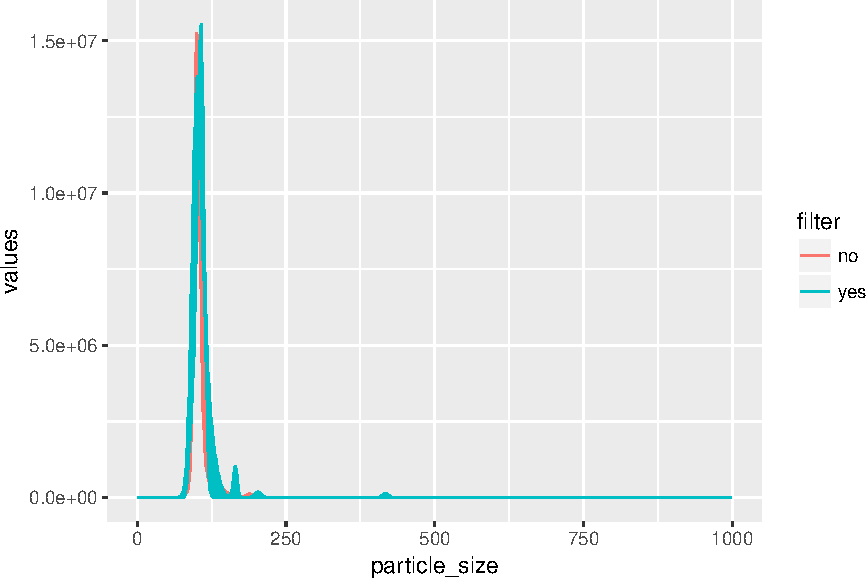
\includegraphics{reproducible_analysis_files/figure-latex/unnamed-chunk-10-1.pdf}

\begin{Shaded}
\begin{Highlighting}[]
\NormalTok{data }\OperatorTok
\StringTok{  }\KeywordTok{filter}\NormalTok{(sample }\OperatorTok{==}\StringTok{ "fluor"}\NormalTok{) }\OperatorTok\StringTok{ }
\StringTok{  }\KeywordTok{ggplot}\NormalTok{(}\KeywordTok{aes}\NormalTok{( }\DataTypeTok{x =}\NormalTok{ particle_size, }\DataTypeTok{y =}\NormalTok{ values, }\DataTypeTok{color =}\NormalTok{ filter))}\OperatorTok{+}
\StringTok{  }\KeywordTok{geom_line}\NormalTok{() }\OperatorTok{+}
\StringTok{  }\KeywordTok{facet_wrap}\NormalTok{(}\OperatorTok{~}\NormalTok{tech_rep)}
\end{Highlighting}
\end{Shaded}

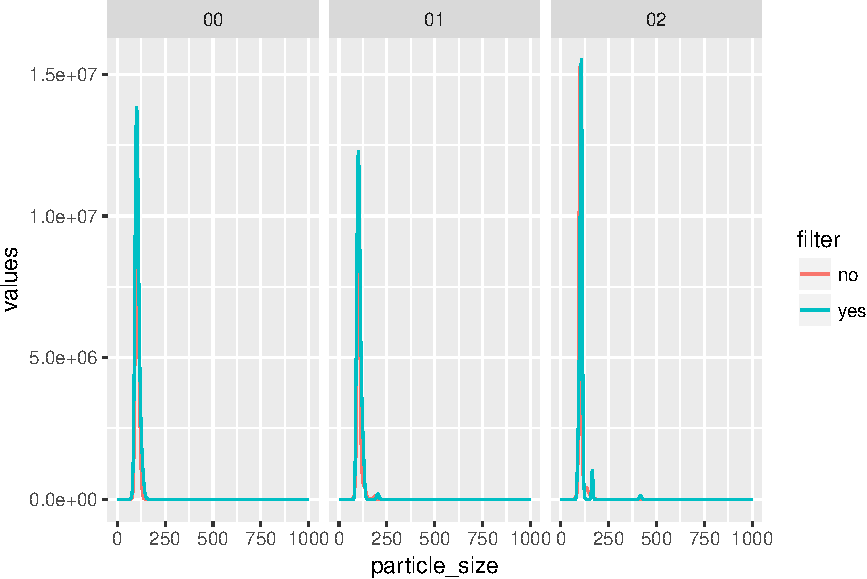
\includegraphics{reproducible_analysis_files/figure-latex/unnamed-chunk-11-1.pdf}

\begin{Shaded}
\begin{Highlighting}[]
\NormalTok{data }\OperatorTok
\StringTok{  }\KeywordTok{filter}\NormalTok{(sample }\OperatorTok{==}\StringTok{ "fluor"} \OperatorTok{&}
\StringTok{         }\NormalTok{particle_size }\OperatorTok{<}\StringTok{ }\DecValTok{300}\NormalTok{) }\OperatorTok\StringTok{ }
\StringTok{  }\KeywordTok{ggplot}\NormalTok{(}\KeywordTok{aes}\NormalTok{( }\DataTypeTok{x =}\NormalTok{ particle_size, }\DataTypeTok{y =}\NormalTok{ values, }\DataTypeTok{color =}\NormalTok{ filter))}\OperatorTok{+}
\StringTok{  }\KeywordTok{geom_line}\NormalTok{() }\OperatorTok{+}
\StringTok{  }\KeywordTok{facet_wrap}\NormalTok{(}\OperatorTok{~}\NormalTok{tech_rep)}
\end{Highlighting}
\end{Shaded}

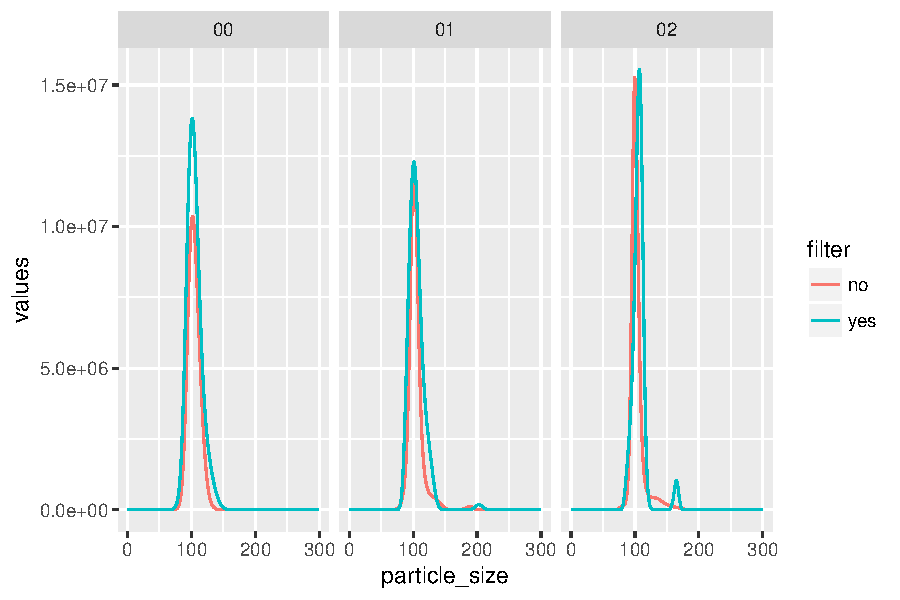
\includegraphics{reproducible_analysis_files/figure-latex/unnamed-chunk-12-1.pdf}

\begin{Shaded}
\begin{Highlighting}[]
\NormalTok{data }\OperatorTok\StringTok{ }
\StringTok{  }\KeywordTok{filter}\NormalTok{(sample }\OperatorTok\StringTok{ }\KeywordTok{c}\NormalTok{(}\StringTok{"100"}\NormalTok{,}\StringTok{"fluor"}\NormalTok{,}\StringTok{"fluorx100"}\NormalTok{),}
\NormalTok{         particle_size }\OperatorTok{<}\StringTok{ }\DecValTok{300}\NormalTok{) }\OperatorTok\StringTok{ }
\StringTok{  }\KeywordTok{ggplot}\NormalTok{(}\KeywordTok{aes}\NormalTok{(}\DataTypeTok{x =}\NormalTok{ particle_size , }\DataTypeTok{y =}\NormalTok{ values, }\DataTypeTok{color =}\NormalTok{ filter))}\OperatorTok{+}
\StringTok{  }\KeywordTok{geom_line}\NormalTok{() }\OperatorTok{+}
\StringTok{  }\KeywordTok{facet_wrap}\NormalTok{(tech_rep}\OperatorTok{~}\NormalTok{sample)}
\end{Highlighting}
\end{Shaded}

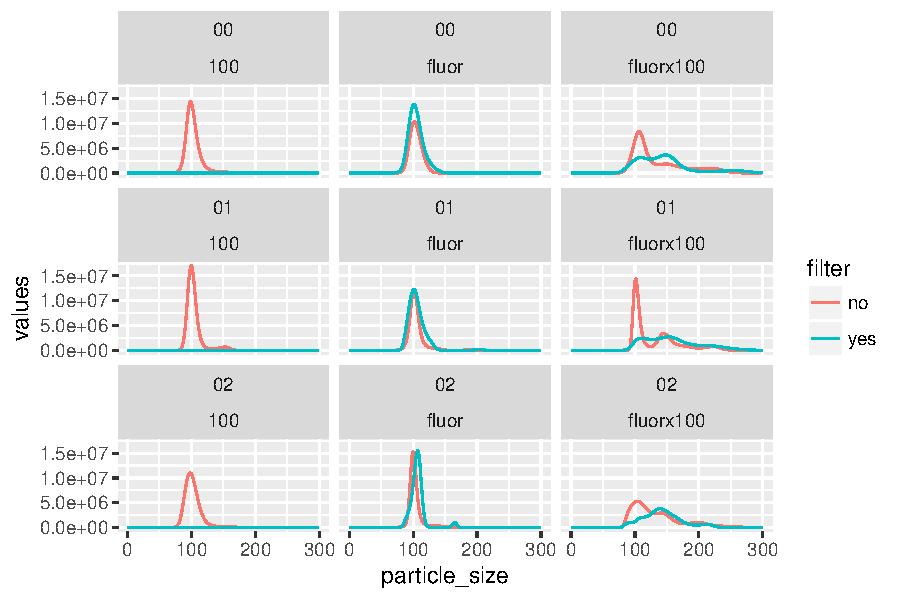
\includegraphics{reproducible_analysis_files/figure-latex/unnamed-chunk-13-1.pdf}

Here are two sample references: {[}1,2{]}.

\section*{References}\label{references}
\addcontentsline{toc}{section}{References}

\hypertarget{refs}{}
\hypertarget{ref-Feynman1963118}{}
1. Feynman R, Vernon Jr. F. The theory of a general quantum system
interacting with a linear dissipative system. Annals of Physics.
1963;24: 118--173.
doi:\href{https://doi.org/10.1016/0003-4916(63)90068-X}{10.1016/0003-4916(63)90068-X}

\hypertarget{ref-Dirac1953888}{}
2. Dirac P. The lorentz transformation and absolute time. Physica.
1953;19: 888--896.
doi:\href{https://doi.org/10.1016/S0031-8914(53)80099-6}{10.1016/S0031-8914(53)80099-6}

\nolinenumbers


\end{document}

